\documentclass{article}
\usepackage{hyperref}
\usepackage{graphicx}
\usepackage{amsmath}
\usepackage{amssymb}
\usepackage{float}
\usepackage{subfig}
\begin{document}

\title{Selected Topics From CS: Assignment 2}
\author{Anirudh Srinivasan (2015A7PS0382H) \\ Bharat Raghunathan (2015AAPS0263H) \\ Nitish Ravishankar (2015A7PS0152H)} 
\maketitle

\tableofcontents

\section{Task 1: Architecture of the Neural Network}
The main aim of the task was to come up with an implementation or representation of the neural network using $C\textrm{++} STL$ containers and 
some variables of our user defined \textbf{Matrix} type
\subsection{Main subtasks presented by the problem}
\begin{enumerate}
	\item Implementing a generic interface:  It was decided to implement a generic template to take the number of layers, the number of nodes in 
	      each layer as input via the 
	      $n\_layers$ variable and $layers\_desc$ array which is an array of size $n\_layers$ and contains the description of each layer, in this 
	      case, the number of nodes in each layer
	\item Random initialization of weights and biases: The weights were initialized with the help of a uniform distribution in the range %$[-1, 1]$ 
	      using an $std::random\_device$ and the default $std::default\_random\_engine$ in $C\textrm{++}$. 
	      The biases are initialized separately and are handled separately throughout the code
\end{enumerate}

\section{Task 2: Feedforward and Backpropagation}
The main aim of this task is to implement a feedforward operation through each layer of the neural network, make a prediction of 
the possible target digit, calculate the \textbf{derivatives/gradient} of the \textbf{cross-entropy} error function with respect to each weight 
using the method of \textbf{backpropagation}.
\subsection{Main subtasks of the problem}
\begin{enumerate}
	\item \textbf{Feedforward}: The value stored at each node in the neural network is a linear combination of the weights of  the previous layer 
	      augmented with the bias term, and the value at the node is activated by using a \textbf{sigmoid} function (except the inputs themselves), 
	      and \textbf{sigmoid} of the final values of the last layer (a 10 x 1 matrix for each example)  is interpreted as the probability of the 
	      given training instance being equal to the $i^{th}$ digit ($i = 0-9$)
	      	      							
	      \begin{align*}
	      	Z^{[1]} & = W^{[1]}X + b^{[1]}         \\
	      	A^{[1]} & = \sigma(Z^{[1]})            \\ \\
	      	Z^{[i]} & = W^{[i]}A^{[i-1]} + b^{[i]} \\
	      	A^{[i]} & = \sigma(Z^{[i]})            \\
	      \end{align*}
	      Time complexity is $O(|w|+|b|)$, where $|w|$ is the total number of weights in the network and $|b|$ is the total number of biases 
	      in the network.
	      	      	      	      	      	      
	\item \textbf{Backpropagation}: Once an iteration of feedforward is over, the error for the output layer is simply the difference between the 
	      actual output matrix and predicted output matrix, which is then used to compute the gradient/derivative for the output layer, then the 
	      error for the ith layer is derived based on the error in the $(i+1)^{th}$ layer, the weights in the ith layer, as well as the derivative
	      of the sigmoid function, which follows the property
	      	      	      	      	      	      
	      $$
	      \frac{d\sigma(x)}{dx} = \sigma(x) \cdot (1-\sigma(x))
	      $$
	      	      	      	      	      	      
	      and hence, the error gets “back propagated” from the last layer to the first layer and the derivative of each layer is then defined by
	      \begin{align*}
	      	dZ^{[n]} & = A^{[n]} - Y                                 \\
	      	dW^{[n]} & = \frac{1}{m}dZ^{[n]}A^{[n-1]^T}              \\
	      	db^{[n]} & = \frac{1}{m}row\_sum(dZ^{[n]})               \\ \\
	      	dZ^{[i]} & = W^{[i+1]^T}dZ^{[i+1]} * \sigma^{'}(Z^{[i]}) \\
	      	dW^{[i]} & = \frac{1}{m}dZ^{[i]}A^{[i-1]^T}              \\
	      	db^{[i]} & = \frac{1}{m}row\_sum(dZ^{[i]})               \\
	      \end{align*}
	      Time complexity is similarly $O(|w|+|b|)$, where $|w|$ is the total number of weights in the network and $|b|$ is the total number of 
	      biases in the network.
	      	      	      	      	      	      
\end{enumerate}

\section{Task 3: Adaptive Gradient and Momentum}
The goal of this task was to implement an \textbf{Adaptive Learning Rate} aided with \textbf{Momentum} to perform an update of the weights, having 
obtained the gradient from backpropagation.

This technique is an iterative approach which tries to reduce the \textbf{misclassification error} in each iteration using the gradient information

Momentum:
\begin{align*}
	v_t    & = \gamma v_{t-1} + \eta \triangledown J(\theta) \\
	\theta & = \theta - v_t                                  \\
\end{align*}

Adagrad:
\begin{align*}
	\theta_{t+1} & = \theta_{t} - \displaystyle \frac{\eta}{\sqrt{G_t+\epsilon}} \odot g_t \\
\end{align*}

where $\eta$ is the learning rate

Combining the two, we gets
\begin{align*}
	v_t    & = \gamma v_{t-1} + \displaystyle \frac{\eta}{\sqrt{G_t+\epsilon}} \odot g_t \\
	\theta & = \theta - v_t                                                              \\
\end{align*}

\section{Results}
\begin{figure}[H]
	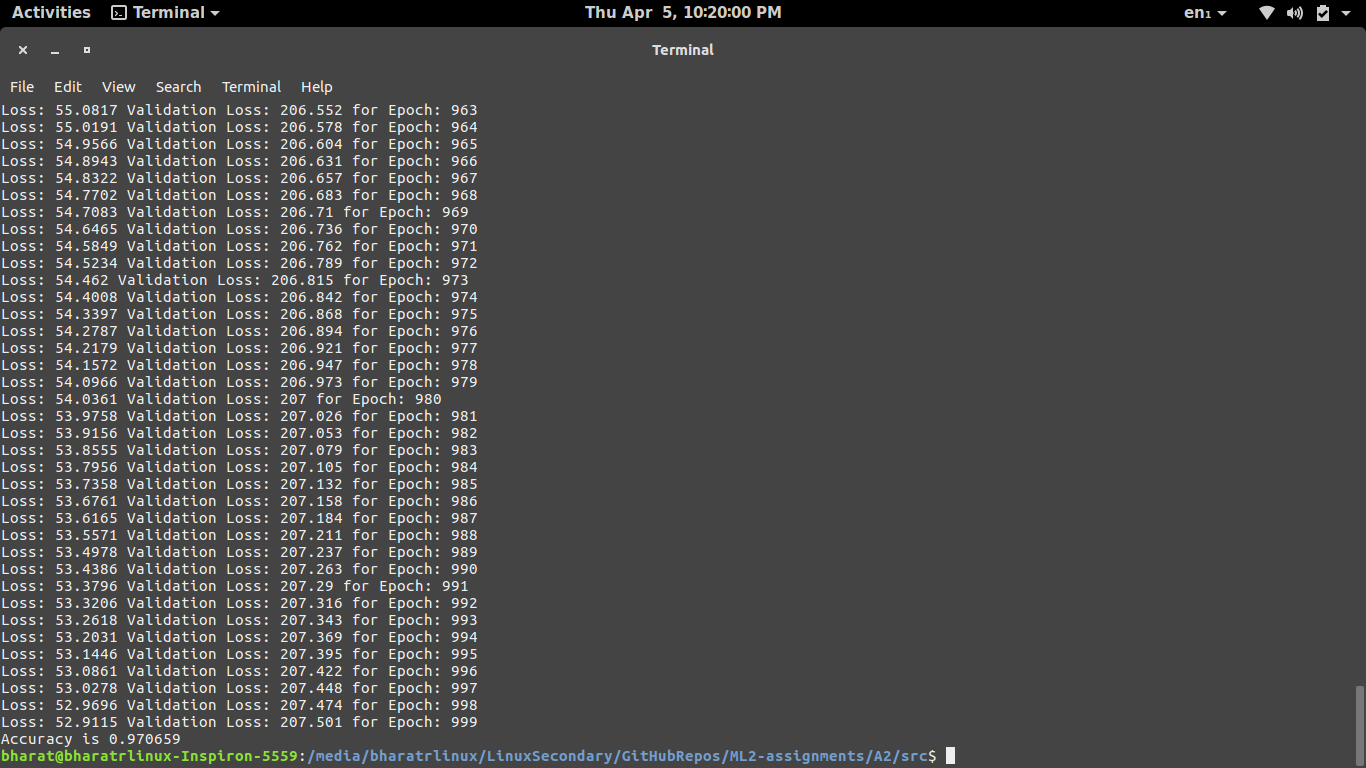
\includegraphics[scale=0.5,trim={0 0.7cm 30cm 10cm},clip]{Results.png}
	\caption{Execution of Program and Display of Results}
\end{figure}
Metric used: \\
$\displaystyle \textrm{Accuracy}= \frac{\textrm{Number of Correct Classifications}}{\textrm{Total number of Test Examples}}$ \\

\subsection{Understanding of Results}
\begin{enumerate}
	
	\item Accuracy of the neural network is over 90\%, indicating that it has almost been able to capture most of the features necessary for 
	      predicting a handwritten digit
	\item More number of hidden layers take a lesser no of epochs to converge and also gives higher Accuracy
	\item Adagrad+Momentum seems to converge faster than plain SGD
\end{enumerate}

\begin{table}[H]
	\begin{tabular}{|c|c|} \hline
		Number of Nodes in Hidden Layer & Accuracy \\ \hline
		5                               & 91.91\%  \\ \hline
		6                               & 93.89\%  \\ \hline
		7                               & 94.31\%  \\ \hline
		8                               & 94.79\%  \\ \hline
		9                               & 95.74\%  \\ \hline
		10                              & 95.98\%  \\ \hline
	\end{tabular}
	\caption{Accuracy for different number of hidden layer nodes}
\end{table}

\begin{figure}[H]
	\subfloat[Accuracy vs Hidden Layer Nodes]{{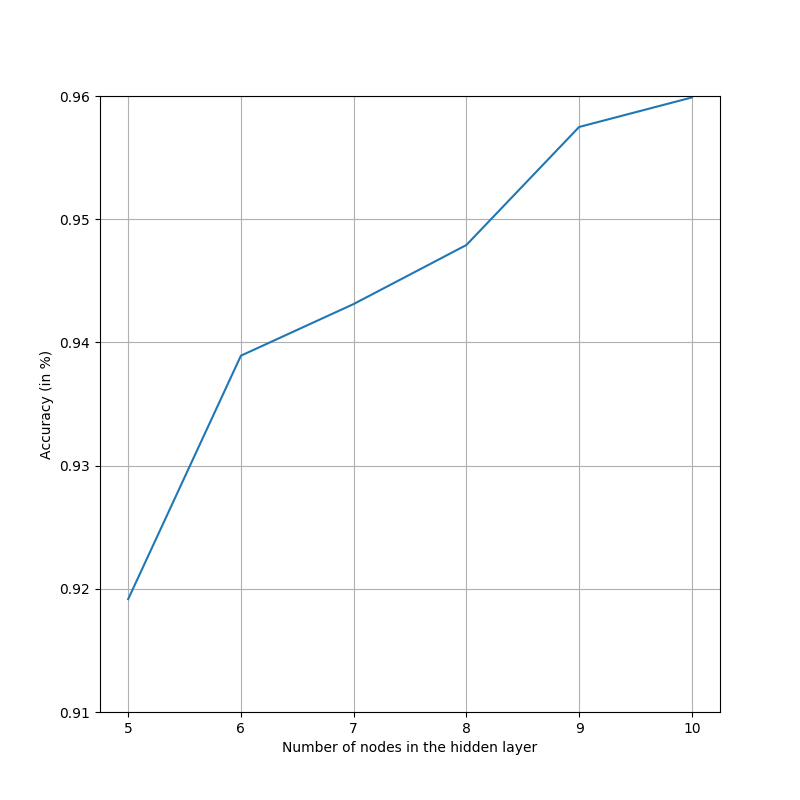
\includegraphics[scale=0.35]{hiddenlayeracc.png}}}
	\subfloat[Epochs vs Hidden Layer Nodes]{{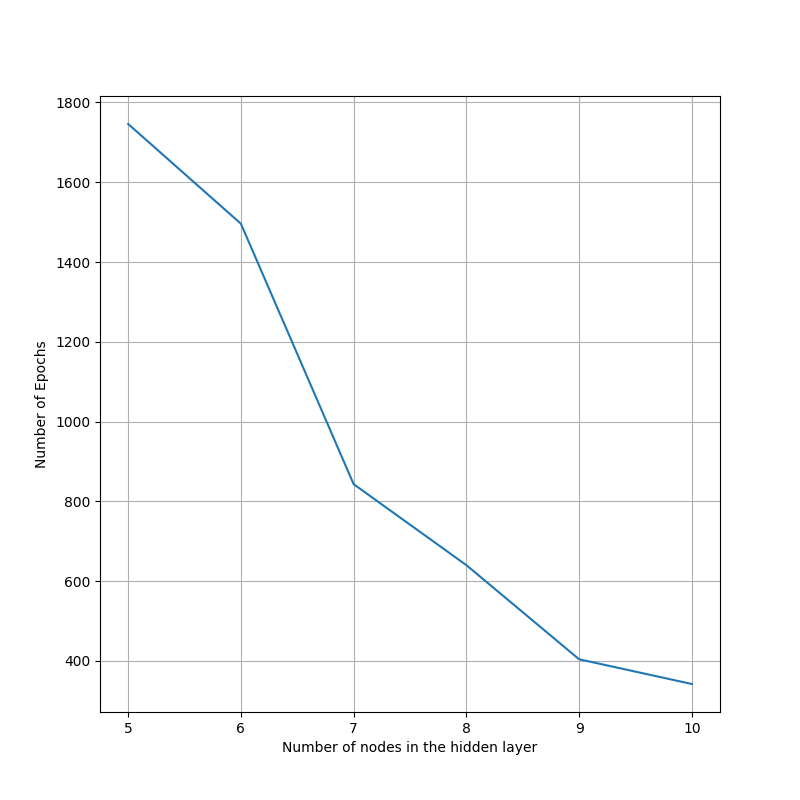
\includegraphics[scale=0.35]{hiddenlayerepochs.png}}}
	\caption{Behaviour on variation of Hidden Layer Nodes}
\end{figure}

\begin{figure}[H]
	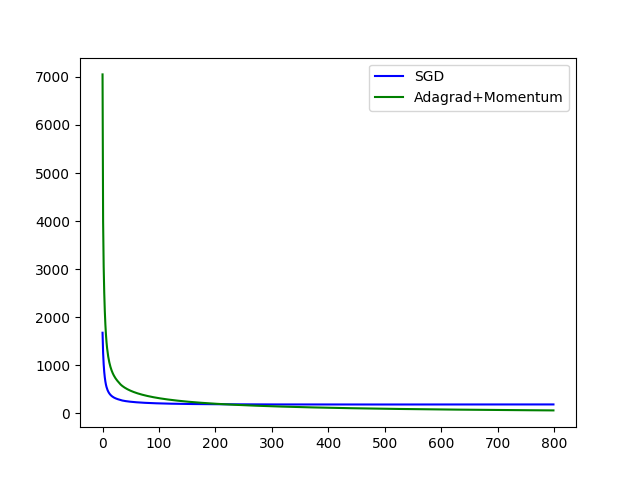
\includegraphics[scale=0.5]{SGDAdagradplot.png}
	\caption{Performance of SGD vs Adagrad+Momentum}
\end{figure}

\appendix
\section{Notation used for Equations}
\begin{align*}
	m        & =\textrm{batch\_size}                                                  \\ 
	Z^{[i]}  & =\textrm{values at node without activation}                            \\
	A^{[i]}  & =\textrm{values at node with activation}                               \\
	dZ^{[i]} & =\textrm{derivatives of } Z^{[i]}                                      \\
	dA^{[i]} & =\textrm{derivatives of } A^{[i]}                                      \\
	W^{[i]}  & =\textrm{weights for transition from layer } i \textrm{ to layer } i+1 \\
	dW^{[i]} & =\textrm{derivatives of } W^{[i]}                                      \\
	b^{[i]}  & =\textrm{biases for transition from layer } i \textrm{ to layer } i+1  \\
	db^{[i]} & =\textrm{derivatives of } b^{[i]}                                      \\
	Y        & = \textrm{target outputs}                                              \\
	X        & = \textrm{inputs}                                                      \\
\end{align*}

\end{document}